\documentclass[pdf]{beamer}
\usepackage{multicol}
\mode<presentation>{}
\usetheme{Warsaw}
\usepackage{subcaption}

%\usepackage{listings}

\title{Clustering por ES, EP e variantes}
\author{Gabriel Evangelista}
\begin{document}

\begin{frame}{Proposta e Metodologia}
	\begin{columns}
		\column{.6\linewidth}
		\textbf{Algoritmos:}
		\begin{itemize}
			\item Evolution Strategies (ES) 
			\item ES - Multimodal - Ilhas constantes
			\item ES - Memético - Baldwin GLA
			\item Evolutionary Programming (EP)
			\item EP - Distribuição de Cauchy (FEP)
		\end{itemize}
	
	
		\textbf{Metodologia:}
		\begin{itemize}
				\item Parâmetros variados comuns:
				\begin{itemize}
					\item $ \mu \in \{10, 30, 60\} $ 
					\item $ \lambda/\mu \in \{3, 5, 7, 10\} $
				\end{itemize}
				\item Parâmetros variados específicos:
				\begin{itemize}
					\item Multimodal:
					\begin{itemize}
						\item $ epoch \in \{10, 50\} $
						\item $ n_{island} \in \{3, 5, 7, 9\} $
					\end{itemize}
					\item Memético: $ epoch \in \{5, 10, 50\} $
					
				\end{itemize}				

		\end{itemize}


		\column{.55\linewidth}
		\begin{itemize}
			\item Limite computacional: $ 5\cdot 10^5 $ avaliações da função custo
			\item Número de Clusters ($ \mathbb{R}^2 $) $ NC \in \{5, 10, 20\} $
			\item Sucesso: tolerância de $5\% \cdot J_{DA} $

			\item Seleção de configuração:
			\begin{itemize}
				\item $ NC \in \{5, 10\} $: $ \ell \xrightarrow{S = True} 10\ell \xrightarrow{best SR} 100 \ell$  
				\item $ NC \in \{20, 30\} $: $ 10\ell \xrightarrow{best SR} 100\ell$ 
			\end{itemize}
					\item Parâmetros analisados: \textit{\textbf{SR}}, \textbf{MBF} e \textit{\textbf{AES}} sobre pelo menos 100 lançamentos
		\end{itemize}		
	\end{columns}
\end{frame}

\begin{frame}{Resultados}
		\begin{figure}
		\begin{subfigure}[t]{\textwidth}
			\centering
			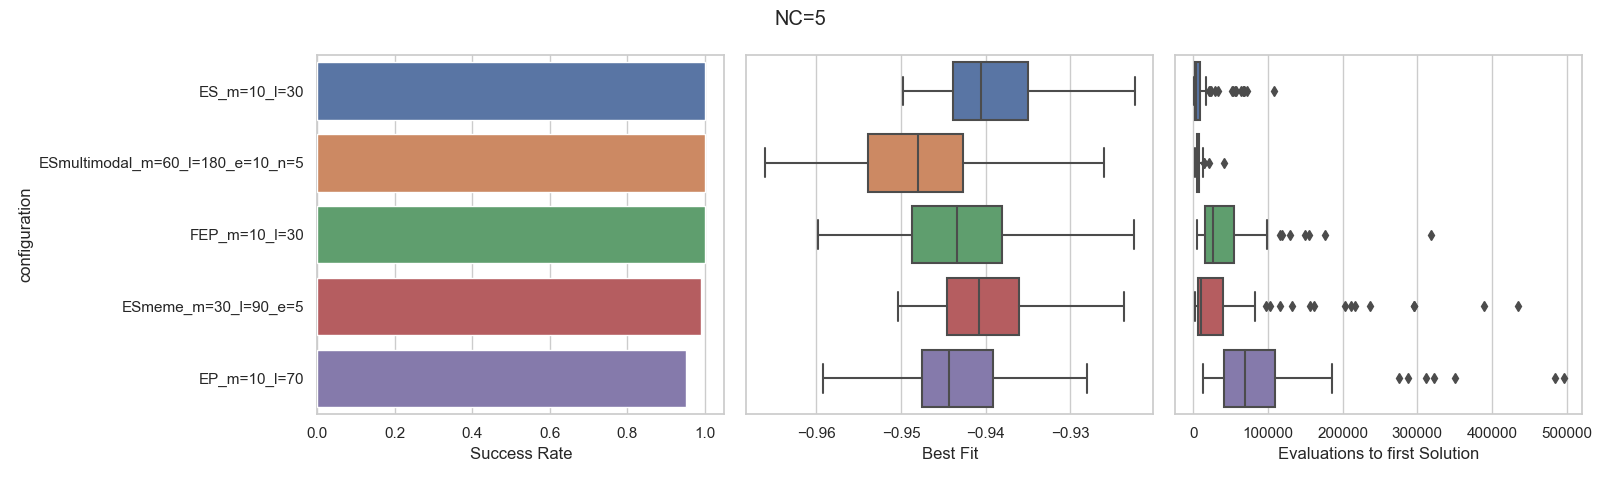
\includegraphics[scale=0.23]{img/NC=5.png}
		\end{subfigure}\
		\begin{subfigure}[t]{\textwidth}
			\centering
			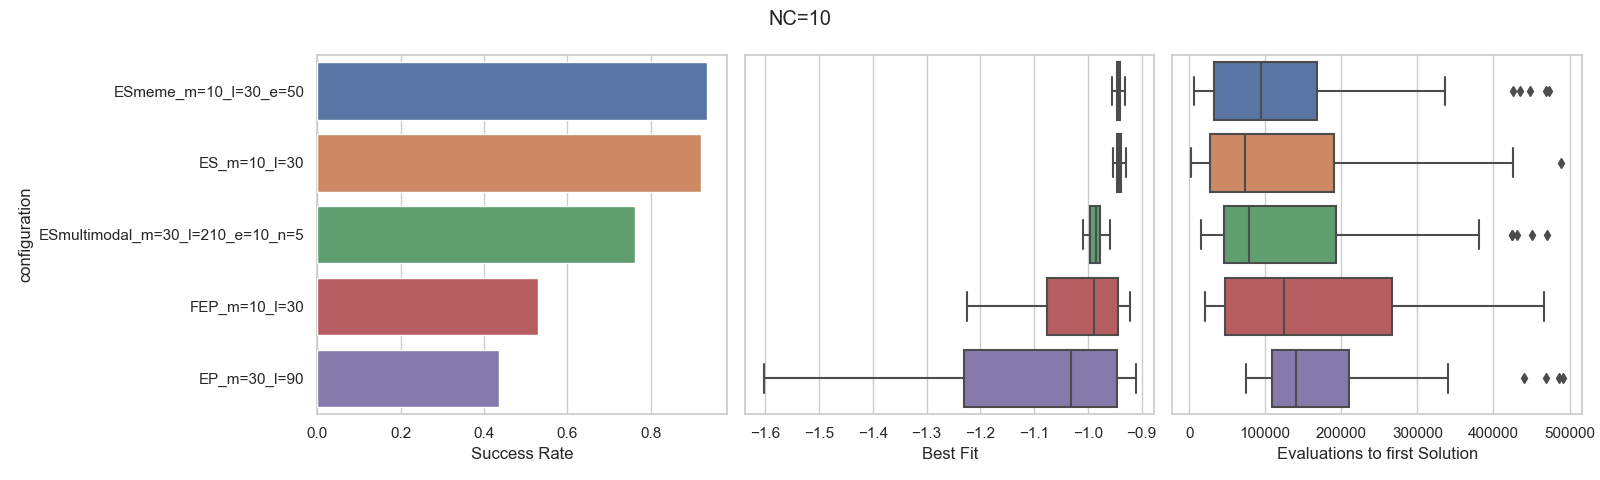
\includegraphics[scale=0.23]{img/NC=10.png}
		\end{subfigure}
		\begin{subfigure}[t]{\textwidth}
			\centering
			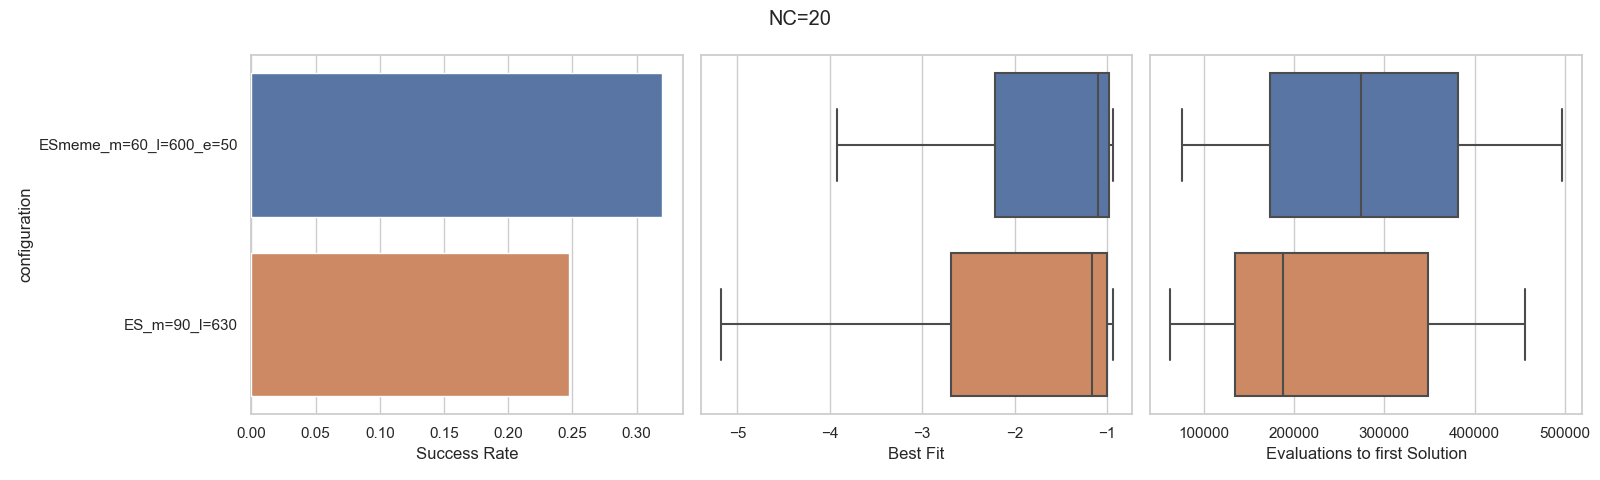
\includegraphics[scale=0.22]{img/NC=20.png}
		\end{subfigure}
	\end{figure}
\end{frame}

\begin{frame}{Resultados}
	\begin{figure}
		\begin{subfigure}[t]{\textwidth}
			\centering
			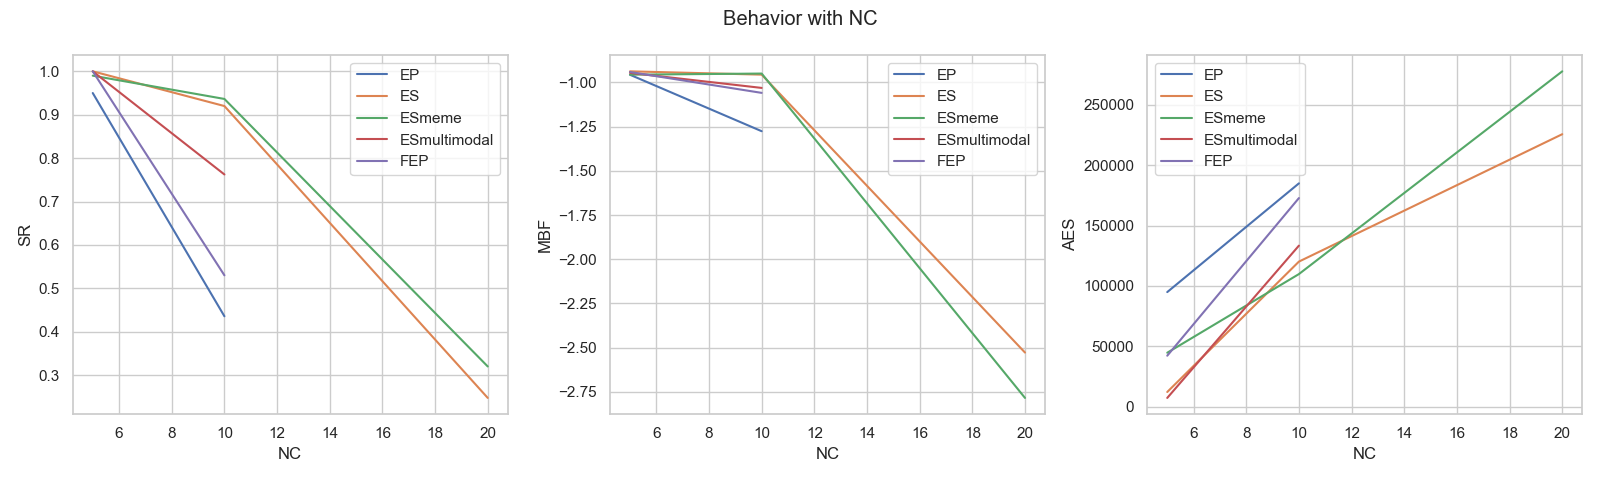
\includegraphics[width=\textwidth]{img/criteria_behavior_with_nc.png}
		\end{subfigure}
		\begin{subfigure}[t]{\textwidth}
			\centering
			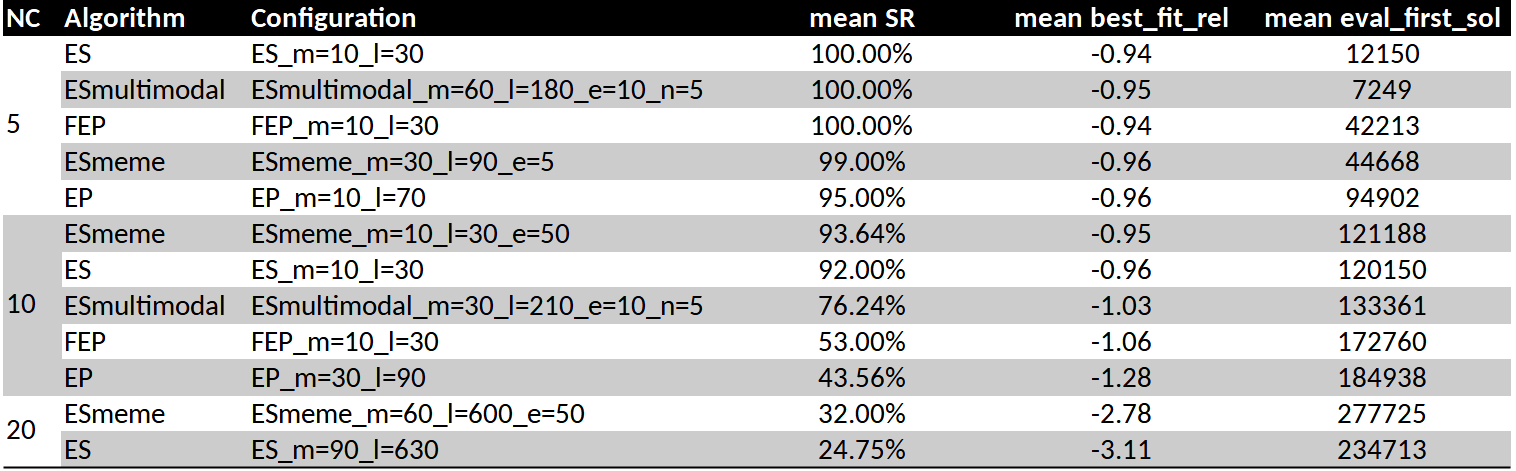
\includegraphics[width=\textwidth]{img/tabela_resumo.png}
		\end{subfigure}
	\end{figure}
\end{frame}

\begin{frame}{Conclusões}
	\begin{itemize}
		\item \textbf{Dificuldade em ganho de escala} de número de \textit{cores} para o problema de \textit{clustering}.
		\item Os algoritmos \textbf{ES} apresentam melhores resultados do que os \textbf{EP} para o problema proposto. Importância da recombinação.
		\item \textbf{FEP} apresenta ganhos de \textbf{SR} em relação a versão \textbf{EP} proposta no problema analisado.
		\item O algoritmo \textbf{ES} memético implementado apresenta melhor comportamento em termos de \textbf{SR} do que a sua variante original. Porém, a análise do gráfico de \textbf{AES} x \textbf{\textit{NC}} sugere que o algoritmo seja mais sensível ao ganho de escala em termos de avaliações do que o original. 

	\end{itemize}
\end{frame}

\end{document}
